\documentclass{theme/uniprthesis}

%%%%%%%%%%%Some Extra Packages%%%%%%%%%%%
\usepackage[italian]{babel}		% To have Italina names in Sections, Figures, Chapters etc.
\usepackage{todonotes}			% To ease the revision
\usepackage{blindtext} 			
\usepackage{ifdraft}
\usepackage{afterpage}
\usepackage{amsmath}
\usepackage{amssymb}
\usepackage{amsfonts}
\usepackage{bbold}
\usepackage{lipsum} 
\usepackage{footmisc}
\usepackage{xcolor}

%%%%% THESIS / TITLE PAGE INFORMATION
% Everybody needs to complete the following:
\title{Titolo della tesi}
\author{Mario Rossi}
\advisor{Giuseppe Verdi}
\college{Dipartimento di Scienze Matematiche, Fisiche e Informatiche}
\degree{Corso di Laurea Triennale/Magistrale in Informatica}
\degreeyears{20xx--20xx}
\serialNumber{0123456}

% Not mandatory fields
% \newcommand{\subTitle}{Titolo in Inglese} %Subtitle, usually the english version of the title

%\newcommand{\advisorSecond}{Prof. Nome2 Cognome2} % For multiple (up to 4) advisors -- if this is not present then also the remaining ones are automatically omitted
%\newcommand{\advisorThird}{Dott. Nome3 Cognome3} % For multiple (up to 4) advisors -- if this is not present then also the remaining ones are automatically omitted
%\newcommand{\advisorFourth}{Dott. Nome4 Cognome4} % For multiple (up to 4) advisors

\newcommand{\coadvisor}{} %For multiple (up to 4) coadvisors -- if this is not present then also the remaining ones are automatically omitted
%\newcommand{\coadvisorSecond}{Prof. co-Nome2 co-Cognome2} % For multiple (up to 4) coadvisors -- if this is not present then also the remaining ones are automatically omitted
%\newcommand{\coadvisorThird}{Dott. co-Nome3 co-Cognome3} % For multiple (up to 4) coadvisors -- if this is not present then also the remaining ones are automatically omitted
%\newcommand{\coadvisorFourth}{Dott. co-Nome4 co-Cognome4} % For multiple (up to 4) coadvisors


\newcommand\blankpage{
    \null
    \thispagestyle{empty}
    \addtocounter{page}{-1}
    \newpage
}

%%%%%%%%%%%%%%%%%%%%%%%%%%%%%%%%%%%%%%%%%%%%%%%%%%%%%%%%%%%%%%%%%%%%%%%%%%%%%%%%%%%%%%%%

\begin{document}

\maketitle
\blankpage % Pagina vuota

%%%%%%%%%%%%%%%%%%%%%%%%%%%%%%%% Citazione
%%%% Commentare questo blocco se non la si vuole mettere
\newpage
\thispagestyle{empty}
\null\vspace{\stretch{1}}
\begin{flushright}
	\textit{Citazione}
\end{flushright}
\vspace{\stretch{3}}\null
\newpage
\blankpage
%%%%%%%%%%%%%%%%%%%%%%%%%%%%%%%% Fine Citazione

%%%%%%%%%%%%%%%%%%%%%%%%%%%%%%%% Dedica
%%%% Commentare questo blocco se non la si vuole mettere
\newpage
\thispagestyle{empty}
\null\vspace{\stretch{1}}
\begin{flushright}
	\textit{Dedica}
\end{flushright}
\vspace{\stretch{3}}\null
\newpage
\blankpage
%%%%%%%%%%%%%%%%%%%%%%%%%%%%%%%% Fine Dedica

%%%%%%%%%%%%%%%%%%%%%%%%%%%%%%%% Indici
\pagestyle{plain}
\pagenumbering{roman}
\tableofcontents

\listoffigures    % Commentare se non vi sono immagini
\listofalgorithms % Commentare se non vi sono algoritmi
\listoftables     % Commentare se non vi sono tabelle

%%%%%%%%%%%%%%%%%%%%%%%%%%%%%%%% Prefazione
\pagenumbering{arabic}
\chapter{Introduzione}\label{chapter:introduzione} 
L'introduzione deve contenere un riassunto del lavoro di Tesi.
In particolare bisogna esprimere chiaramente e molto sinteticamente: contesto dello studio, motivazioni, contributo e conclusioni.
Bisogna quindi fare un sommario dello studio ad alto livello, fornendo le intuizioni senza ricadere in dettagli tecnici.
Anche lo stile dovrebbe essere più discorsivo rispetto alle parti tecniche della tesi.


	
%%%%%%%%%%%%%%%%%%%%%%%%%%%%%%%% Contenuto
\pagestyle{fancy}
\chapter{Formattazione}\label{chapter:formattazione}
Prima di introdurre il capitolo si può scrivere una breve introduzione su ciò che si andrà ad affrontare.
In questo capitolo, per esempio, saranno presentati alcuni esempi di formattazione degli oggetti più comuni di una Tesi in informatica.


\section{Capitoli, Sezioni e Sottosezioni}\label{sec:cap_sec_subsec}
Capitoli, sezioni e sottosezioni devono essere usate appropriatamente e non sostituire elenchi puntanti.
In particolare, i Capitoli devono riguardare macro-argomenti della tesi; ad esempio \textbf{Background}, \textbf{Obiettivi}, \textbf{Progettazione/Implementazione} e \textbf{Risultati}.
Questi capitoli sono semplicemente una traccia bisogna adattare a seconda delle esigenze.

Le sezioni invece devono riguardare argomenti all'interno della macro-area definita dal capitolo.
Ad esempio se più tecniche sono state utilizzate durante la tesi si può suddividere il capitolo \textbf{Progettazione/Implementazione} in sezioni, ognuna riguardante una delle tecniche sperimentate.

Le sottosezioni infine si possono utilizzare per descrivere concetti distinti all'interno di ogni sezione, ognuno dei quali deve avere una sua identità.
Ogni sottosezione deve avere un motivo per essere definita e non semplicemente separare parti di uno stesso discorso, per quello c'è l'indentazione (doppio ``a capo'' per separare parti distinte dello stesso paragrafo e ``$\backslash\backslash$'' per separare due paragrafi).

\subsection{Esempio di sottosezione}\label{subsec:es_subsec}
\blindtext

\section{Esempi di immagini}\label{sec:images}
Di seguito alcuni esempi di immagini.
Figura~\ref{fig:one} presenta una singola immagine con ancoraggio ``\textbf{ht}" che chiede al altex di lasciare la figura dove si trova, se possibile, e altrimenti di metterla in alto alla pagina.
Figura~\ref{fig:two} presenta una singola immagine con due sotto-figure con ancoraggio ``\textbf{ht}".
Figura~\ref{fig:three} presenta una singola immagine con tre sotto-figure con ancoraggio ``\textbf{H}" che forza l'immagine nel posto scelto dall'utente, questa opzione è sconsigliata a meno di necessità particolari.
Ogni volta che un'immagine è inserita è buona norma citarla nel testo, altrimenti l'immagine non avrebbe un chiaro significato.
Nel caso delle sotto-immagini si possono citare anche loro, ad esempio Figura~\ref{fig:lev1} è composta da altre due sotto-figure.
\begin{figure}[ht]
	\centering
	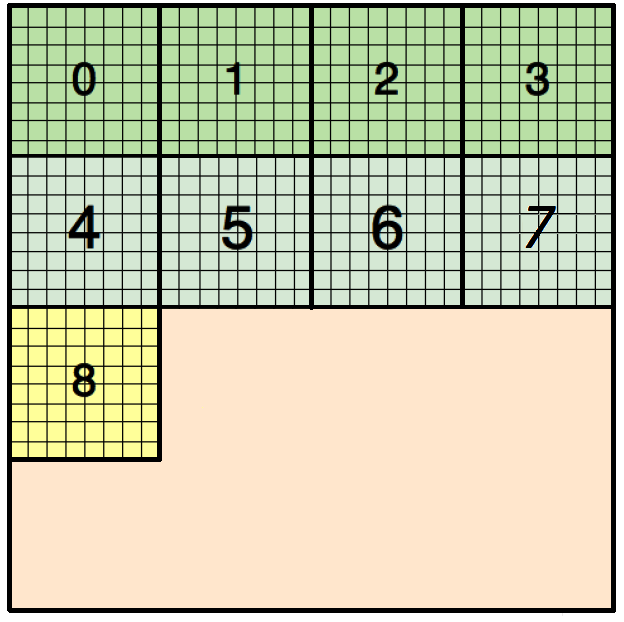
\includegraphics[width=0.3\textwidth]{immagini/block_on_grid.png}
	\caption{Figura con singola immagine}
	\label{fig:one}
\end{figure}

\begin{figure}[ht]
	\centering
	\begin{subfigure}{0.3\textwidth}
		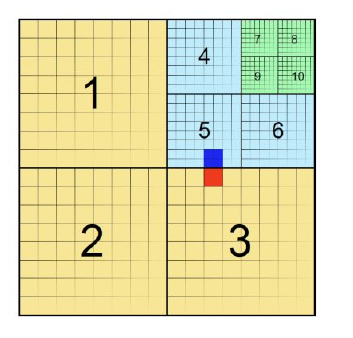
\includegraphics[width=1.0\textwidth]{immagini/disoposizione_blocchi_fisica.png}
		\caption{Disposizione fisica dei blocchi}
	\end{subfigure}%
	\begin{subfigure}{0.3\textwidth}
		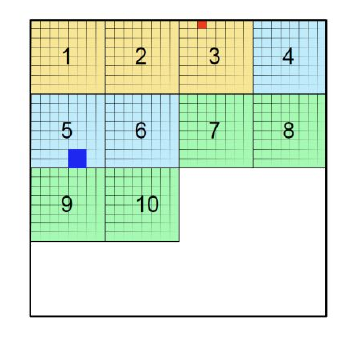
\includegraphics[width=1.0\textwidth]{immagini/disoposizione_blocchi_logica.png}
		\caption{Disposizione logica dei blocchi}
	\end{subfigure}
	\caption{Figura con due immagini}
	\label{fig:two}
\end{figure}


\begin{figure}[H]
	\centering
	\begin{subfigure}{0.5\textwidth}
		\centering
		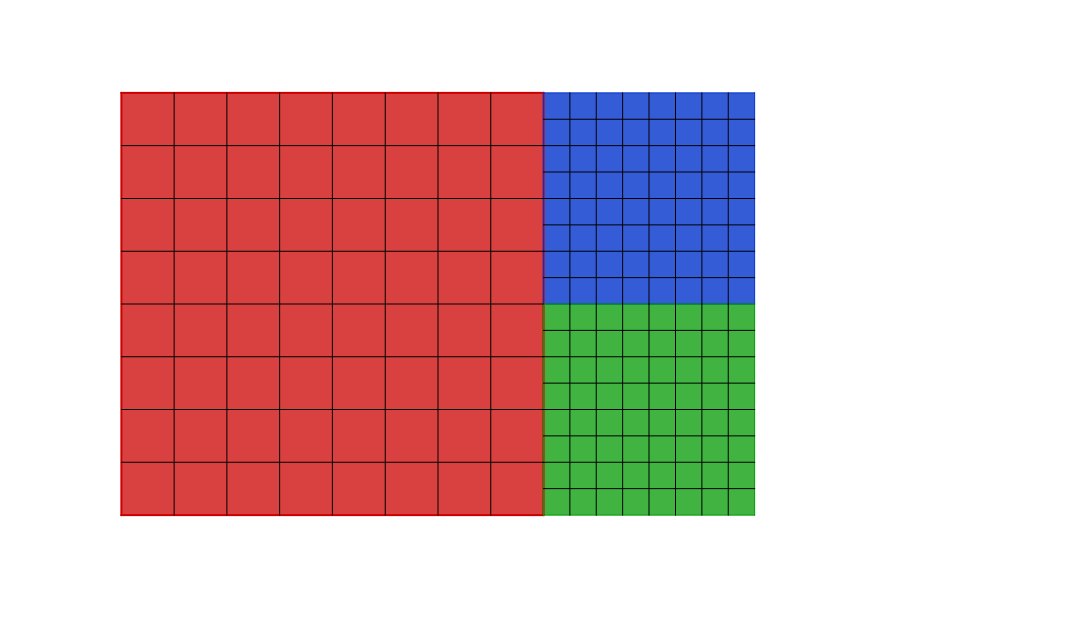
\includegraphics[width=0.7\linewidth]{immagini/lev_less1.png}
		\caption{\textit{lev} = -1\newline}
		\label{fig:test1}
	\end{subfigure}%
	\begin{subfigure}{0.5\textwidth}
		\centering
		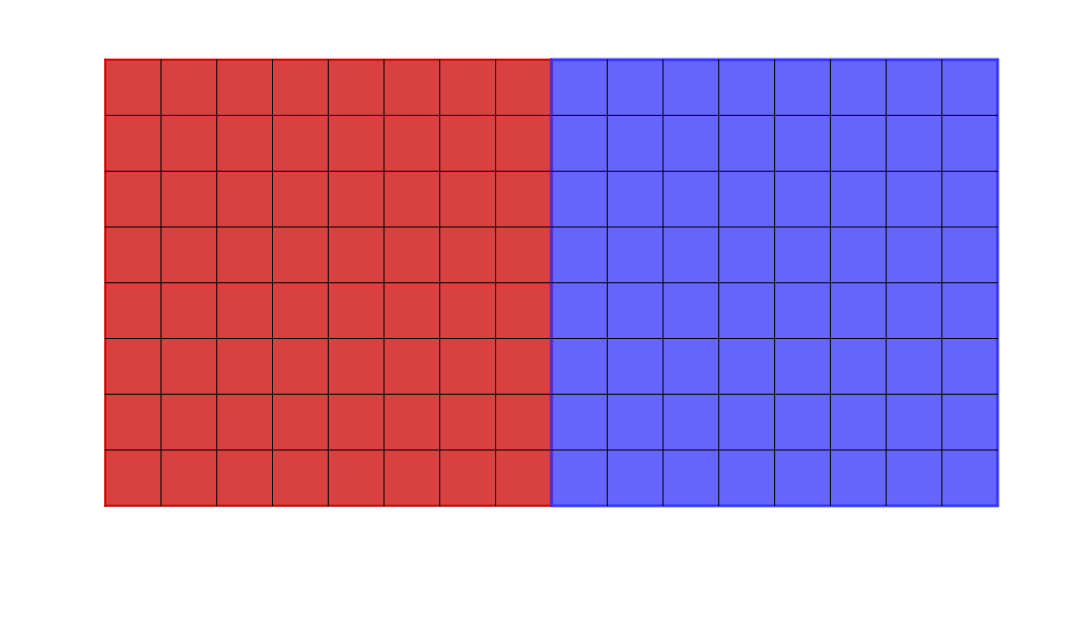
\includegraphics[width=0.7\linewidth]{immagini/lev0.png}
		\caption{\textit{lev} = 0\newline}
		\label{fig:test2}
	\end{subfigure}
	\begin{subfigure}{0.7\textwidth}
		\centering
		\begin{subfigure}{0.5\textwidth}
			\centering
			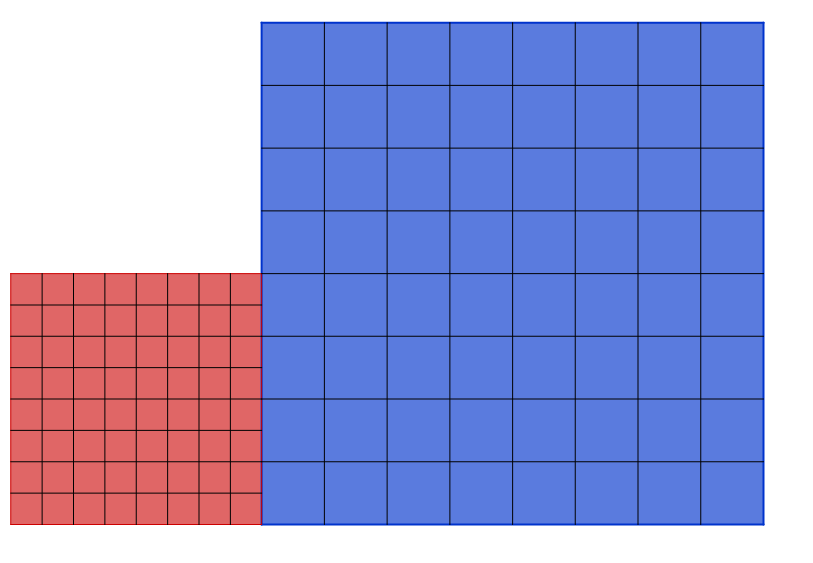
\includegraphics[width=0.5\linewidth]{immagini/bloccomaggiore1.png}
		\end{subfigure}%
		\begin{subfigure}{0.5\textwidth}
			\centering
			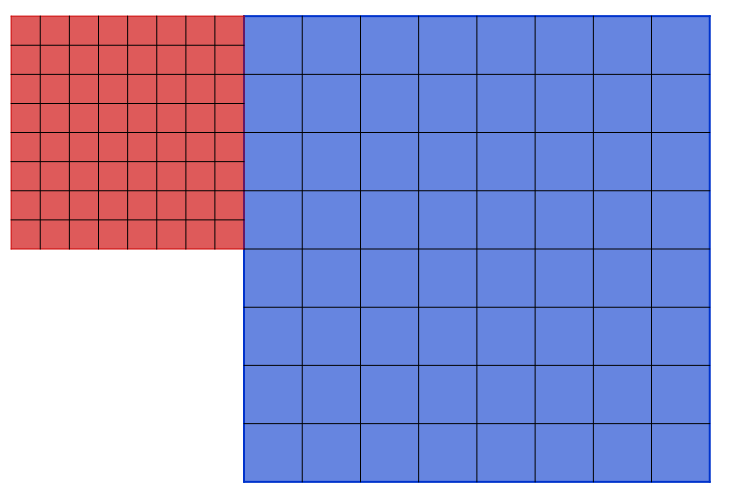
\includegraphics[width=0.5\linewidth]{immagini/bloccomaggiore2.png}
		\end{subfigure}
		\caption{\textit{lev} = 1}
		\label{fig:lev1}
	\end{subfigure}
	\caption{Figura con tre immagini (di cui una composta da due sotto-immagini)}
	\label{fig:three}
\end{figure}

\section{Esempi di Codice e Misc.}\label{sec:code}
Alcuni esempi di codice, definizioni, tabelle e altro.

\begin{algorithm}[ht]
	\caption{Esempio di pseudo-codice}
	\label{alg:Prim_Mst}
	\begin{algorithmic}[1]
		\Statex
		\Function{MST-Prim}{grafo G, funzione\_peso $\omega$, nodo\_radice r}\\
		\State{\textit{Q}: coda di priorita contenente tutti i vertici in \textit{V}}
		\For{ogni \textit{u} $\in$ V(G)}
		\Let{\textit{u.key}}{$\infty$}
		\Let{\textit{u.}$\pi$}{\textit{NIL}} 
		\EndFor
		\Let{\textit{r.key}}{0}
		\Let{\textit{Q}}{\textit{V(G)}}
		\While{\textit{Q} $\neq$ 0}
		\Let{\textit{u}}{EXTRACT-MIN(\textit{Q})}
		\For{ogni \textit{v} $\in$ \textit{G.Adj[u]}}
		\If{$v \in Q$ and $\omega(u,v) < v.key$}
		\Let{\textit{v.key}}{$\omega(u,v)$}
		\Let{\textit{v.}$\pi$}{\textit{v}}
		\EndIf
		\EndFor
		\EndWhile
		\State \Return{}
		\EndFunction
	\end{algorithmic}
\end{algorithm}

\begin{algorithm}[]
	\caption{Caption}
    \label{lst:kintegersetinizio}
    \begin{lstlisting}[style=custom, language=C]
	struct Block
	{
		int id_block;
		char resolution;
		int id_subdomain;
		int key;
		bool in_other_subdomain;
		struct neigh_t neighbors[4];
	};
\end{lstlisting}
\end{algorithm}



\begin{algorithm}[ht]
	\caption{Esempio di codice imperativo}
	\label{alg:my_prim_multi}
	\begin{algorithmic}[1]
		\Statex
		\Function{PRIM\_MULTI-MST}{roots\_list \textit{roots}, array\_Block \textit{adjacency\_list}}
		
		\State{\color{blue}{//Inizializzazione di tutti i vertici}}
		\For{ogni \textit{u} $\in$ \textit{adjacency\_list}}
		\Let{\textit{u.key}}{$\infty$}
		\Let{\textit{u.id\_subdomains}}{\textit{NIL}}
		\Let{\textit{u.in\_other\_subdomain}}{FALSE} 
		\EndFor
		
		\State{\color{blue}{//Inizializzazione di tutte le radici}}
		\Let{\textit{i}}{0}
		\For{ogni \textit{r} $\in$ \textit{roots}}
		\Let{\textit{r.key}}{0}
		\Let{\textit{r.id\_subdomains}}{\textit{i}}
		\Let{\textit{i}}{$i+1$}
		\EndFor
		\State{\textit{Q}: coda di priorita ordinata in base al campo 
			\textit{key}}
		\Let{\textit{Q}}{\textit{roots}}
		\Let{\textit{count}}{0}
		
		\While{count $<$ \textit{adjacency\_list.size}}
		\Let{\textit{u}}{EXTRACT-MIN(\textit{Q})}
		
		\If{!(\textit{u.in\_other\_subdomain})}
		\State{\color{blue}{//Essendo il minimo viene aggiunto definitivamente}}
		\Let{\textit{u.in\_other\_subdomain}}{TRUE}
		\State{\color{blue}{//Si analizzano i vicini}}
		\For{ogni \textit{v} $\in$ \textit{u.neighbors}}
		\State{\color{blue}{//In questo caso specifico il peso di ogni arco vale 1}}
		\If{$v \in adjacency\_list$ and ($u.key+1) < v.key$}
		\Let{\textit{v.key}}{$u.key+1$}
		\Let{\textit{v.subdomains}}{\textit{u.subdomains}}
		\Let{\textit{count}}{\textit{count} + 1}
		\EndIf
		\EndFor
		\EndIf
		\EndWhile
		\State \Return{}
		\EndFunction
	\end{algorithmic}
\end{algorithm}

\begin{algorithm}[ht]
	\caption{esempio di algoritmo in C++}
	\label{lst:genic_mpi}
	\begin{lstlisting}[style=custom, language=C]
		#include "mpi.h"
		
		
		
		main(int argc, char** argv){
			
			
			
			//Nessuna chiamata a funzioni MPI prima di questa
			MPI_Init(&argc, &argv);
			
			
			
			MPI_Finalize();
			//Nessuna chiamata a funzioni MPI dopo questa
			
			
		}	
	\end{lstlisting}
\end{algorithm}

\begin{defn}[Esempio di Definizione]
	Un piccolo esempio di definizione
\end{defn}

\begin{table}[ht]
	\centering
	\resizebox{0.99\linewidth}{!}{
		\begin{tabular}{|c|c|c|c|c|c|c|c|c|c|c|}
			\hline
			CT scan &01&02&03&04&05&06&07&08&09&10 \\
			\hline
			Input arteries (n.) &66&175&76&134&198&172&154&108&91&65 \\
			\hline
			Labeling time (s)&19.13&87.38&26.11&47.08&90.89&356.95&303.77&91.95&16.01&21.88 \\
			\hline
			Grounding time (s)&9.76&52.45&9.57&22.88&70.34&47.52&37.44&17.98&10.61&8.04 \\
			\hline
			Optimum time (s)&6.66&31.05&14.67&20.63&15.2&29.17&54.71&61.03&4.28&7.24 \\
			\hline
		\end{tabular}
	}

	\caption{Esempio di tabella}
	\label{tab:perf}
\end{table}


\section{Citazioni}
Durante la scrittura della Tesi è necessario fornire i riferimenti bibliografici che hanno permesso la stesura della tesi stessa.
Questo si ottiene semplicemente tramite l'utilizzo del comando ``cite'' che prende come argomento la label di una delle entry nel file .bib.
Quindi per citare una qualunque fonte, ad esempio ``Artificial Intelligence - A Modern Approach", si può fare \cite{modernApproach} ($\backslash\text{cite}\{\text{modernApproach}\}$).
Questo leggerà la referenza nel file .bib che ha come label ``cormen".
Per citare più riferimenti contemporaneamente basta sperare le varie labels con una virgola come segue \cite{gelfond1998action,modernApproach,durfee1999distributed,de2003resource,allen2009complexity,bernstein2002complexity}.
Le reference non citate non appariranno in bibliografia.
\href{https://dblp.uni-trier.de/}{dblp} e \href{https://scholar.google.com/}{Google Scholar} sono siti nei quali estrarre la reference per bibtex per un lavoro di cui si conosce solo il titolo, ad esempio.

\section{Footnote}
È possibile utilizzare le footnote\footnote{Test della footnote} con il comando\footnote{Test della footnote 2} $\backslash\text{footnote}\{\text{ ... }\}$.
\chapter{Background}\label{chapter:background}
\Blindtext %Dummy Text - remove
\Blindtext %Dummy Text - remove

%%%%%%%%%%%%%%%%%%%%%%%%%%%%%%%% Conclusioni
\pagestyle{plain}
\chapter*{Conclusione} %Se si cambia il Titolo cambiare anche la riga successiva così che appia corretto nell'conclusione
\addcontentsline{toc}{chapter}{Conclusione} %Per far apparire Introduzione nell'indice (Il nome deve rispecchiare quello del chapter)
Conclusione che riassume il lavoro svolto ed eventuali lavori futuri.

\blindtext %Dummy Text - remove
\blindtext %Dummy Text - remove

%%%%%%%%%%%%%%%%%%%%%%%%%%%%%%%% Appendici
\appendix
\chapter{Appendice di Esempio}
\Blindtext

%%%%%%%%%%%%%%%%%%%%%%%%%%%%%%%% Bibliografia
\bibliographystyle{plain} % {apalike, plain, IEEEtran, ACM-Reference-Format} -- Scegliere lo stile preferito
\cleardoublepage
\addcontentsline{toc}{chapter}{\bibname}
\bibliography{./bibliografia}

%%%%%%%%%%%%%%%%%%%%%%%%%%%%%%%% Ringraziamenti
\chapter*{Ringraziamenti}
\thispagestyle{empty}
\pagestyle{empty}



\Blindtext %Dummy Text - remove
\newpage
\thispagestyle{empty}
\null\vspace{\stretch{1}}
\vspace{\stretch{3}}\null
\newpage

\blankpage
\end{document}